For this analysis, we had three in-house annotators manually label the
object segmentations in our dataset. The annotators were provided the
original image (for reference) and the object segmentation and asked
to assign a single category to the segment out of $7$ possible
categories: animal, building, device, furniture, nature, person, and
vehicle. We chose these categories so that a wide range of object
classes could be covered. For example, category ``device'' includes
objects like utensils, bottles, and televisions, while ``nature'' includes objects like trees, mountains, and flowers, and “vehicle” contains cars, bikes, and airplanes. Figure \ref{fig:avgMem} shows the distribution of the memorability scores of all $7$ object categories in our dataset.

\begin{figure}[b]
\centering
\subfigure{\centering 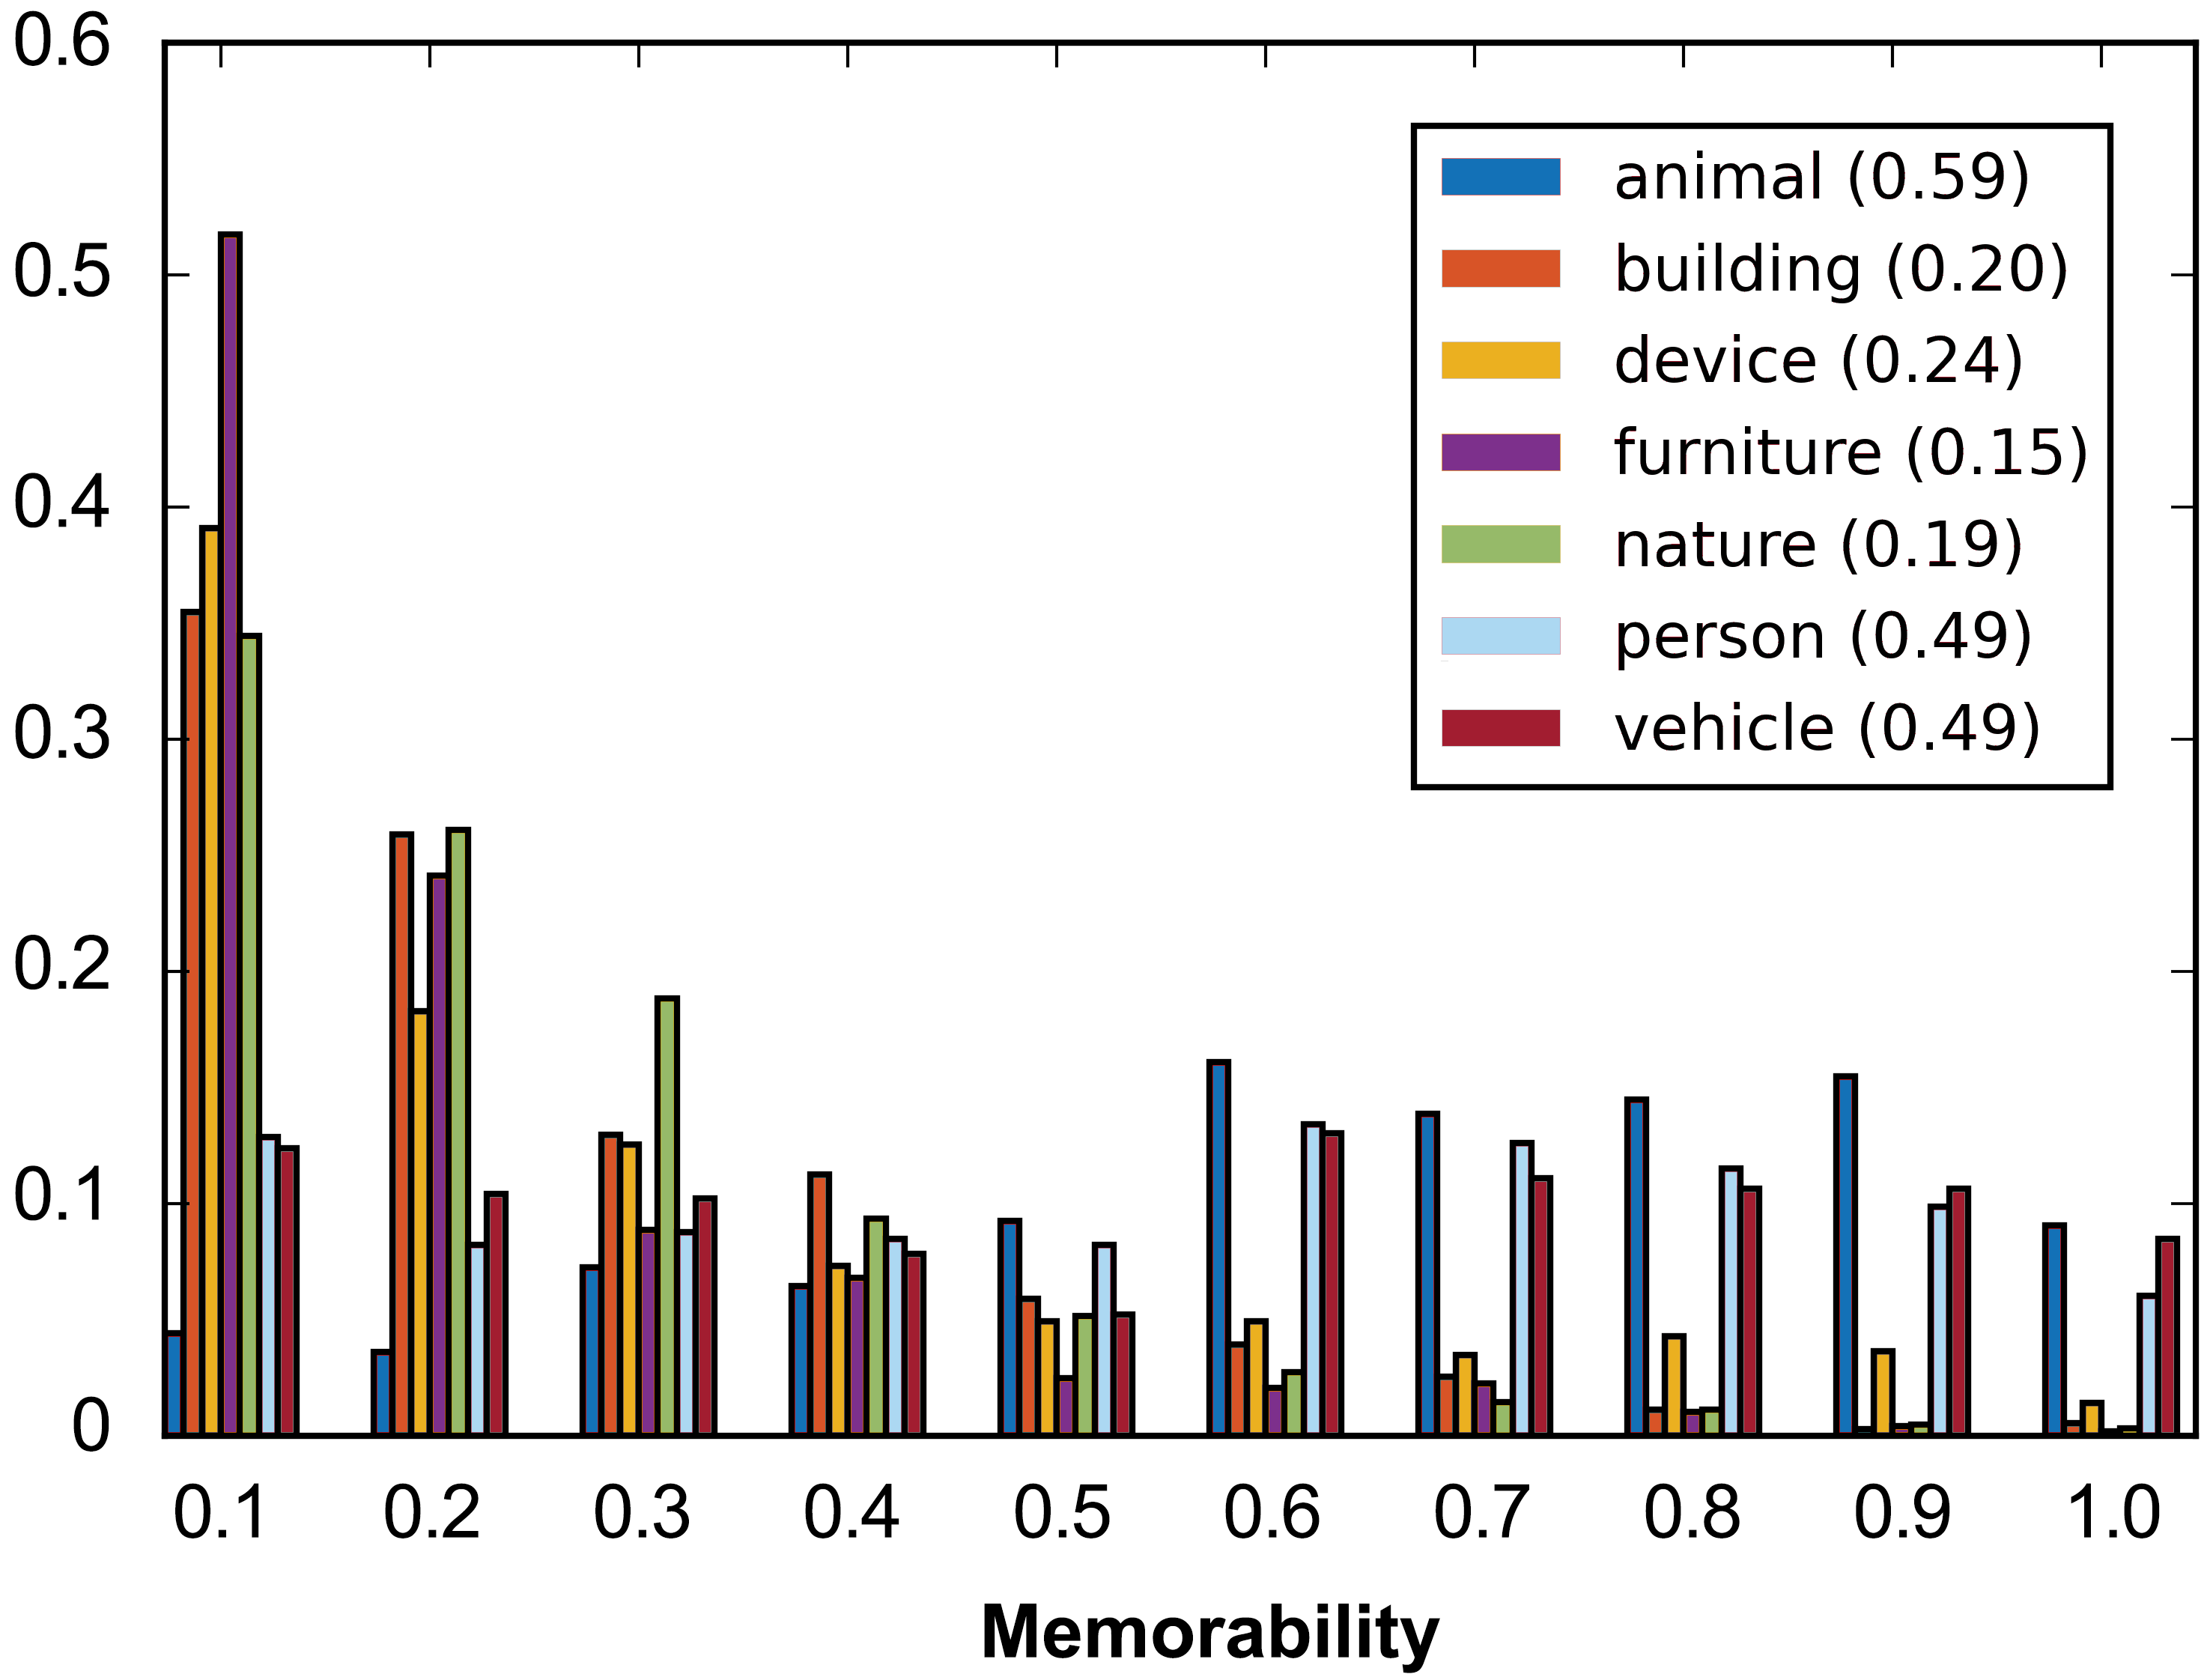
\includegraphics[width=0.47\textwidth]{figures/results/obLabel/memScore_dist3.png}}
\vspace{-5mm}\caption{\footnotesize\textbf{Some object categories are more memorable than others.} Categories like furniture, nature, building, and device tend to have a large majority of objects with very low memorability scores. Objects belonging to animal, person, and vehicle categories are remembered more often.}\label{fig:avgMem}
\end{figure}

Results in Figure \ref{fig:avgMem} give a sense of how  memorability changes across different object categories. Animal, person, and vehicle are all highly memorable classes each associated with  an average memorability score greater than or close to $0.5$. Interestingly, all other categories have an average memorability lower than $0.25$, indicating that humans do not remember objects from these categories very well. In particular, furniture is the least memorable category with an average score of only $0.14$. This is possibly due to the fact that most objects in the furniture, nature, and building categories either appear mostly in the background or are occluded, which likely decreases their memorability significantly. In contrast, objects from the animal, person, and vehicle categories appear mostly in the foreground, leading to a higher memorability score on average. Interestingly, the most memorable objects from building, furniture, and nature tend to have an average memorability in the range of $0.4 - 0.8$, whereas the score of the most memorable objects from person, animal and vehicle is higher than $0.9$. %This is particularly interesting as these top objects are not occluded and most of them tend to appear in the foreground.
While the differences in the memorability of different object categories could be driven due to factors like occlusion, size, background/foreground, or photographic bias, the distribution in Figure \ref{fig:avgMem} suggests that humans remember some object classes such as person, animal, and vehicle irrespective of external nuisance factors and these categories are \textit{intrinsically} more memorable than others.


%distribution of the most memorable objects within each class suggest that memorability could be an intrinsic property of an object class.  The right side of the figure presents an interesting analysis This analysis is particularly interesting as these top objects are not occluded and most of them tend to appear in the foreground. The top $20$ most memorable objects from person, animal and vehicle have memorability higher than $0.90$ whereas the average memorability of the top $20$ objects from building, furniture, and nature is lesser than $0.70$. While the differences in the memorability of different classes could be driven primarily due to factors like occlusion, size, background/foreground, the results in table \ref{tab:avgMem} suggest that memorability could be an intrinsic property of an object class and some object classes like person, animal, vehicle are in general intrinsically more memorable than classes like furniture, nature etc.
%

